\subsection{Limited Cacheability}
\begin{figure}
\begin{center}
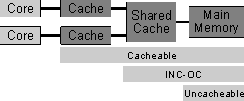
\includegraphics[width=0.5\textwidth]{\chapterdirectory/figure/handling_it/cacheability.pdf}
\end{center}
\caption{Cacheability Levels}%
\label{fig:handling_it:cacheability}
\end{figure}

One approach to the control of interference generated by cache coherence is to
limit which memory elements are affected by it. \cite{bansal2019cache} argues
for letting developers indicate, upon memory allocation, whether to allow the
new memory elements to be either cacheable as usual, not cacheable at all, or
only cacheable in caches shared by all cores (refered to as \texttt{INC-OC}).
Figure~\ref{fig:handling_it:cacheability} summarizes where memory elements can
be stored depending on the attribute they have been given.  \texttt{INC-OC},
which is the main contribution of the paper, is intended to remove these memory
elements from the cache coherence while not having to suffer the full cost of a
cacheless system upon their access. This does indeed result in more easily
predicted memory accesses for these particular memory elements, as they now
behave as they would in a single core system running concurrent programs:
another core/program may still evict them (either directly, or by allocating
more memory and triggering the automated eviction policy), but the possibles
system-wide states of those restricted memory elements (and thus possible
access latencies) are much fewer that they would otherwise be. This can thus
allow approaches for the analysis of memory latencies in single-core system to
be applied to these memory elements, a problem for which the available
literature is more prominent than for multi-core systems, with the added issue
of bandwidth sharing between the cores for access to that last-level cache.

As for limitations, the most oblivious one is that this is only applicable to
systems which do indeed implement a last-level cache being accessed by every
core. Furthermore, the addition of a new type of memory leads to hardware
modifications: translation look-aside buffers need to take into consideration a
new attribute, and so do all sent memory access queries. The authors argue that
some of these hardware modifications can sometimes be minimized through the use
of the architecture's instructions, and that this approach has the advantage of
being entirely orthogonal to the cache coherence mechanisms, thus not requiring
any modification of the admittedly complex coherence controllers.

In effect, the approach presented in \cite{bansal2019cache} requires some
hardware, as well minor operating system and hypervisor, modifications, in
order to let designers simplify the analysis, and lower the variation, of the
access time for any memory elements they choose. This does come at the cost of
the speed at which these memory elements are accessed, and it does require the
designer make a decision as to which memory elements should be handled this way.
